\documentclass{article}
\usepackage{graphicx}
\usepackage{amsmath}
\usepackage{amsfonts}
\usepackage{bookmark}
\usepackage{booktabs}
\usepackage{exercises}
\graphicspath{ {./images/8.5} }
\usepackage{indentfirst}
\usepackage{amsthm}
\usepackage{yhmath}
\usepackage{geometry}
\usepackage{placeins}
\usepackage{csquotes}
\usepackage{pgfplots}
\newcommand*{\oldneg}{\mathord{\sim}}
\newcommand\showdiv[1]{\overline{\smash{)}#1}}
\newcommand\Mydiv[1]{%
\smash{\raise.3ex\hbox{$\big)$}}\mkern-8mu
        \overline{\enspace\strut#1}}
\setlength{\tabcolsep}{5pt}
\theoremstyle{definition}
\newtheorem{definition}{Definition}

\setlength{\parindent}{.5in}
\setlength{\parskip}{12pt}
\renewcommand{\arraystretch}{2}
\geometry{margin=1in}
\newcommand{\?}{\stackrel{?}{=}}
\pgfplotsset{width=7cm,compat=1.18}\usepgfplotslibrary{statistics}

\title{8.5 Answers}
\begin{document}
\maketitle

\section*{1}
The points $(-2,0)$ and $(2,0)$ in the graph at the right are the vertices of the hyperbola. The line segment joining these two points is the 
transverse axis.

\section*{2}
An ellipse is defined to be the set of all points such that the sum of the distances between the point and two points, called the foci, is constant. A hyperbola is 
defined to be the set of all points such that the difference of the distances between the point and two points, called the foci, is constant. Thus both the definition of an 
ellipse and that of a hyperbola involve fixed points called the foci, but the ellipse keeps the sum of the distances between a point and the foci constant, whereas a 
hyperbola keeps the difference of the distances between a point and the foci constant.

\section*{4}
We are given the equation $\frac{x^2}{9}-\frac{y^2}{36}=1$, meaning $a=\sqrt{9}=3$ and $b=\sqrt{36}=6$. Thus the vertices are $(\pm 3,0)$. 
Because the $x^2$ term comes first in the equation, the 
transverse axis is horizontal. We know that asymptotes are $y=\pm\frac{3}{6}=\pm\frac{1}{2}$. We know $a$ and $b$, meaning we can find $c$:
\[ c^2=3^2+6^2 \] \[ c=\sqrt{45}=3\sqrt{5} \] and thus the foci are $(\pm 3\sqrt{5},0)$:\newline
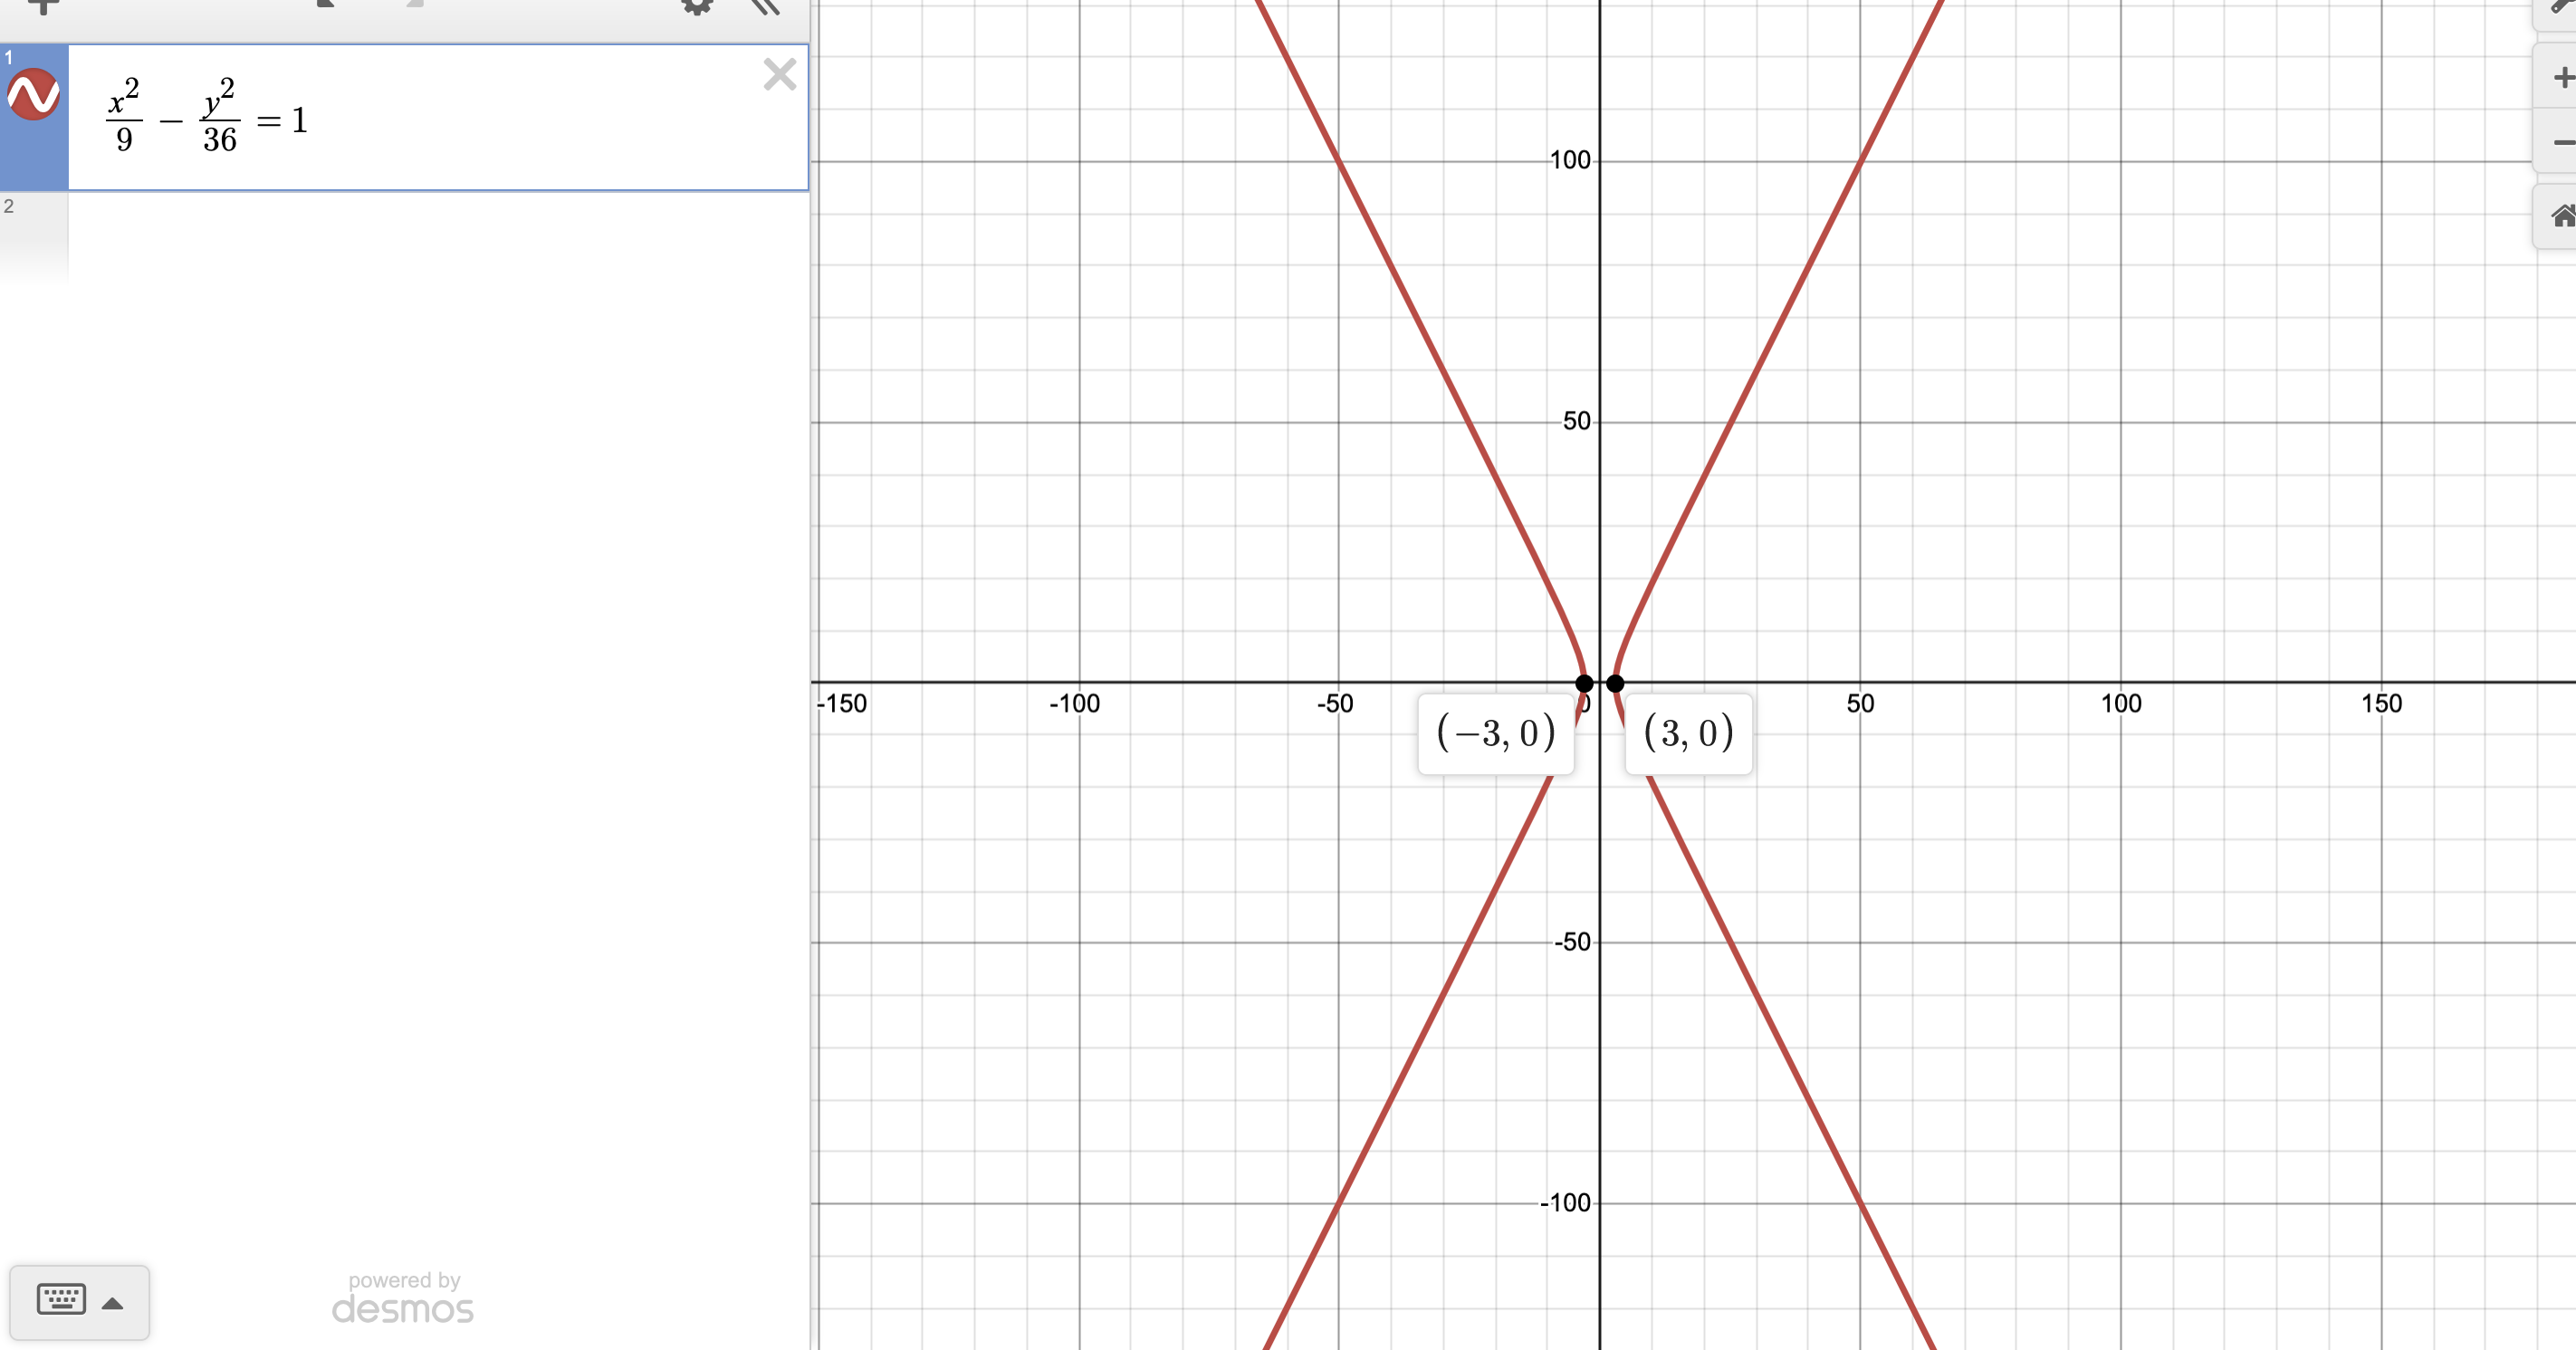
\includegraphics[width = 4in]{4}

\section*{7}
We are given the equation $\frac{y^2}{196}-\frac{x^2}{100}=1$, meaning $a=\sqrt{196}=14$ and $b=\sqrt{100}=10$. Because the $y^2$ term comes first in the equation, 
the transverse axis is vertical, and the vertices are $(0,\pm 14)$. Also, the asymptotes are $y=\pm\frac{10}{14}=\pm\frac{5}{7}$. We know $a$ and $b$, meaning we 
can find $c$:
\[ c^2=14^2+10^2 \]
\[ c=\sqrt{396}=6\sqrt{11} \]
and thus the foci are $(0,\pm 6\sqrt{11})$:\newline
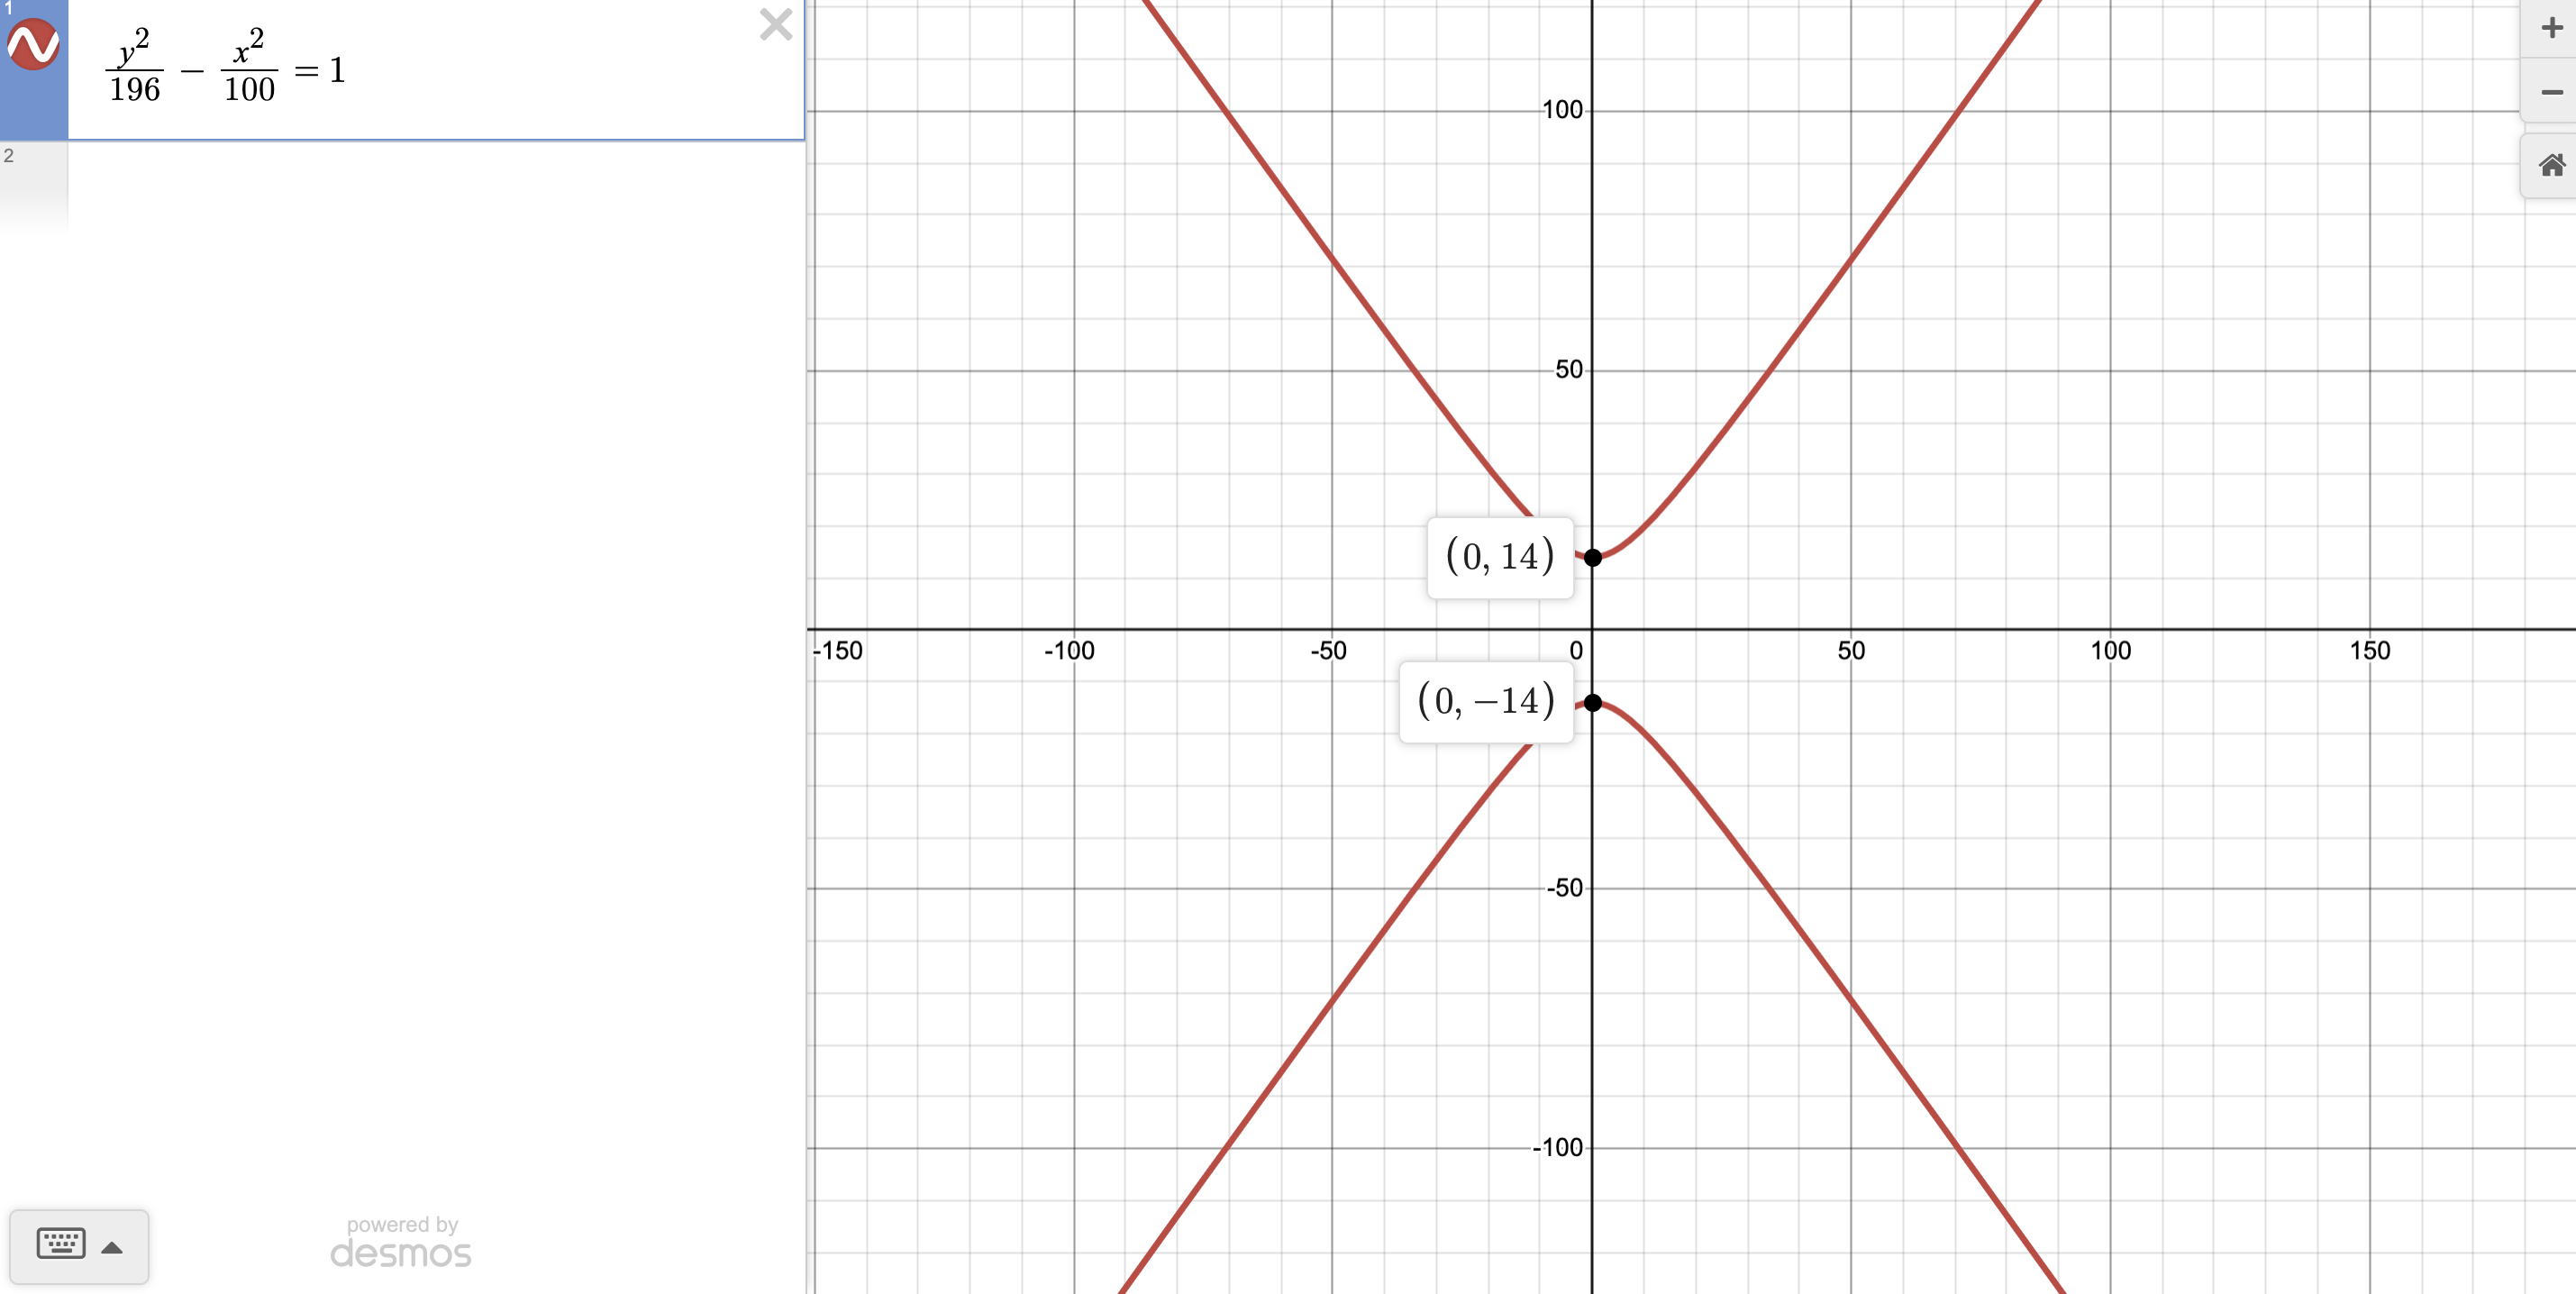
\includegraphics[width = 4in]{7}

\section*{10}
We are given the equation \[ 49x^2-4y^2=196 \] \[ \frac{x^2}{4}-\frac{y^2}{49}=1 \] meaning $a=\sqrt{4}=2$ and $b=\sqrt{49}=7$. Because the $x^2$ term comes first 
in the equation, the transverse axis is horizontal, and the vertices are $(\pm 2,0)$. Also, the asymptotes are $y=\pm\frac{2}{7}$. We know $a$ and $b$, meaning we can 
find $c$:
\[ c^2=2^2+7^2 \] \[ c=\sqrt{53} \]
and thus the foci are $(\pm\sqrt{53},0)$:\newline
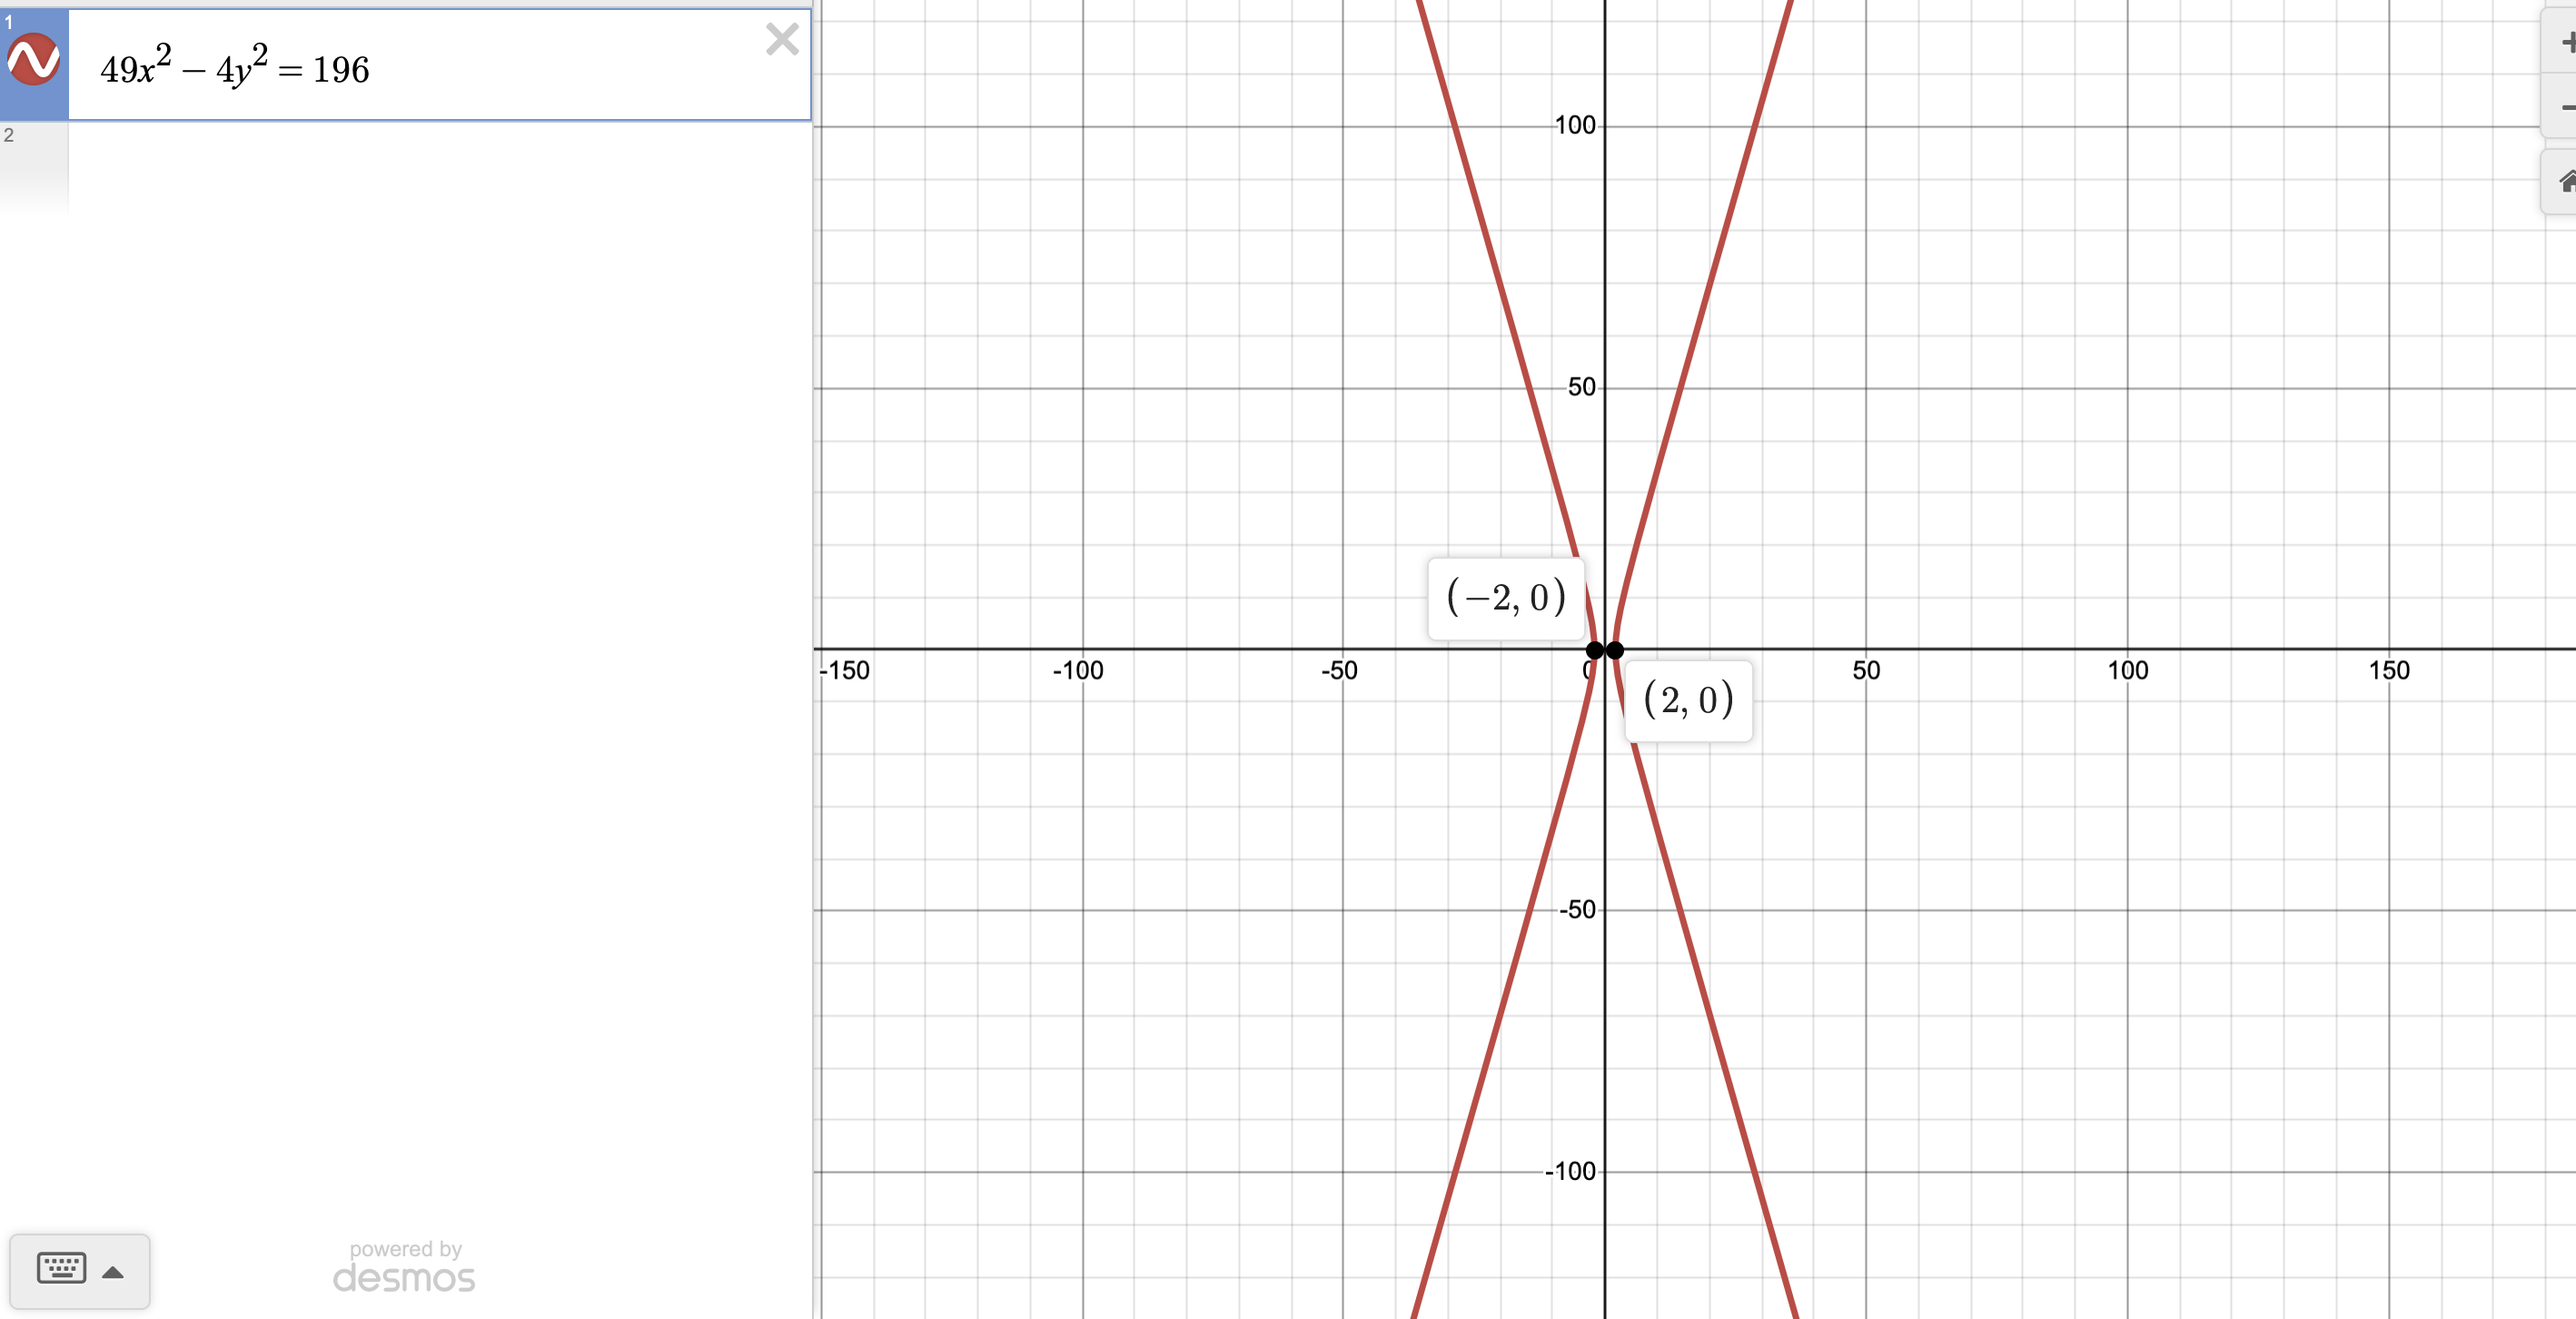
\includegraphics[width = 4in]{10}

\section*{14}
We are given the equation \[ 49y^2-100x^2=4900 \] \[ \frac{y^2}{100}-\frac{x^2}{49}=100 \] meaning $a=\sqrt{100}=10$ and $b=\sqrt{49}=7$. Because the $y^2$ term 
comes frist in the equation, the transverse axis is vertical, and the vertices are $(0,\pm 10)$. Also, the asymptotes are $y=\pm\frac{7}{10}$. We know $a$ and $b$, meaning 
we can find $c$:
\[ c^2=10^2+7^2 \] \[ c=\sqrt{149} \] and thus the foci are $(0,\pm\sqrt{149})$:\newline
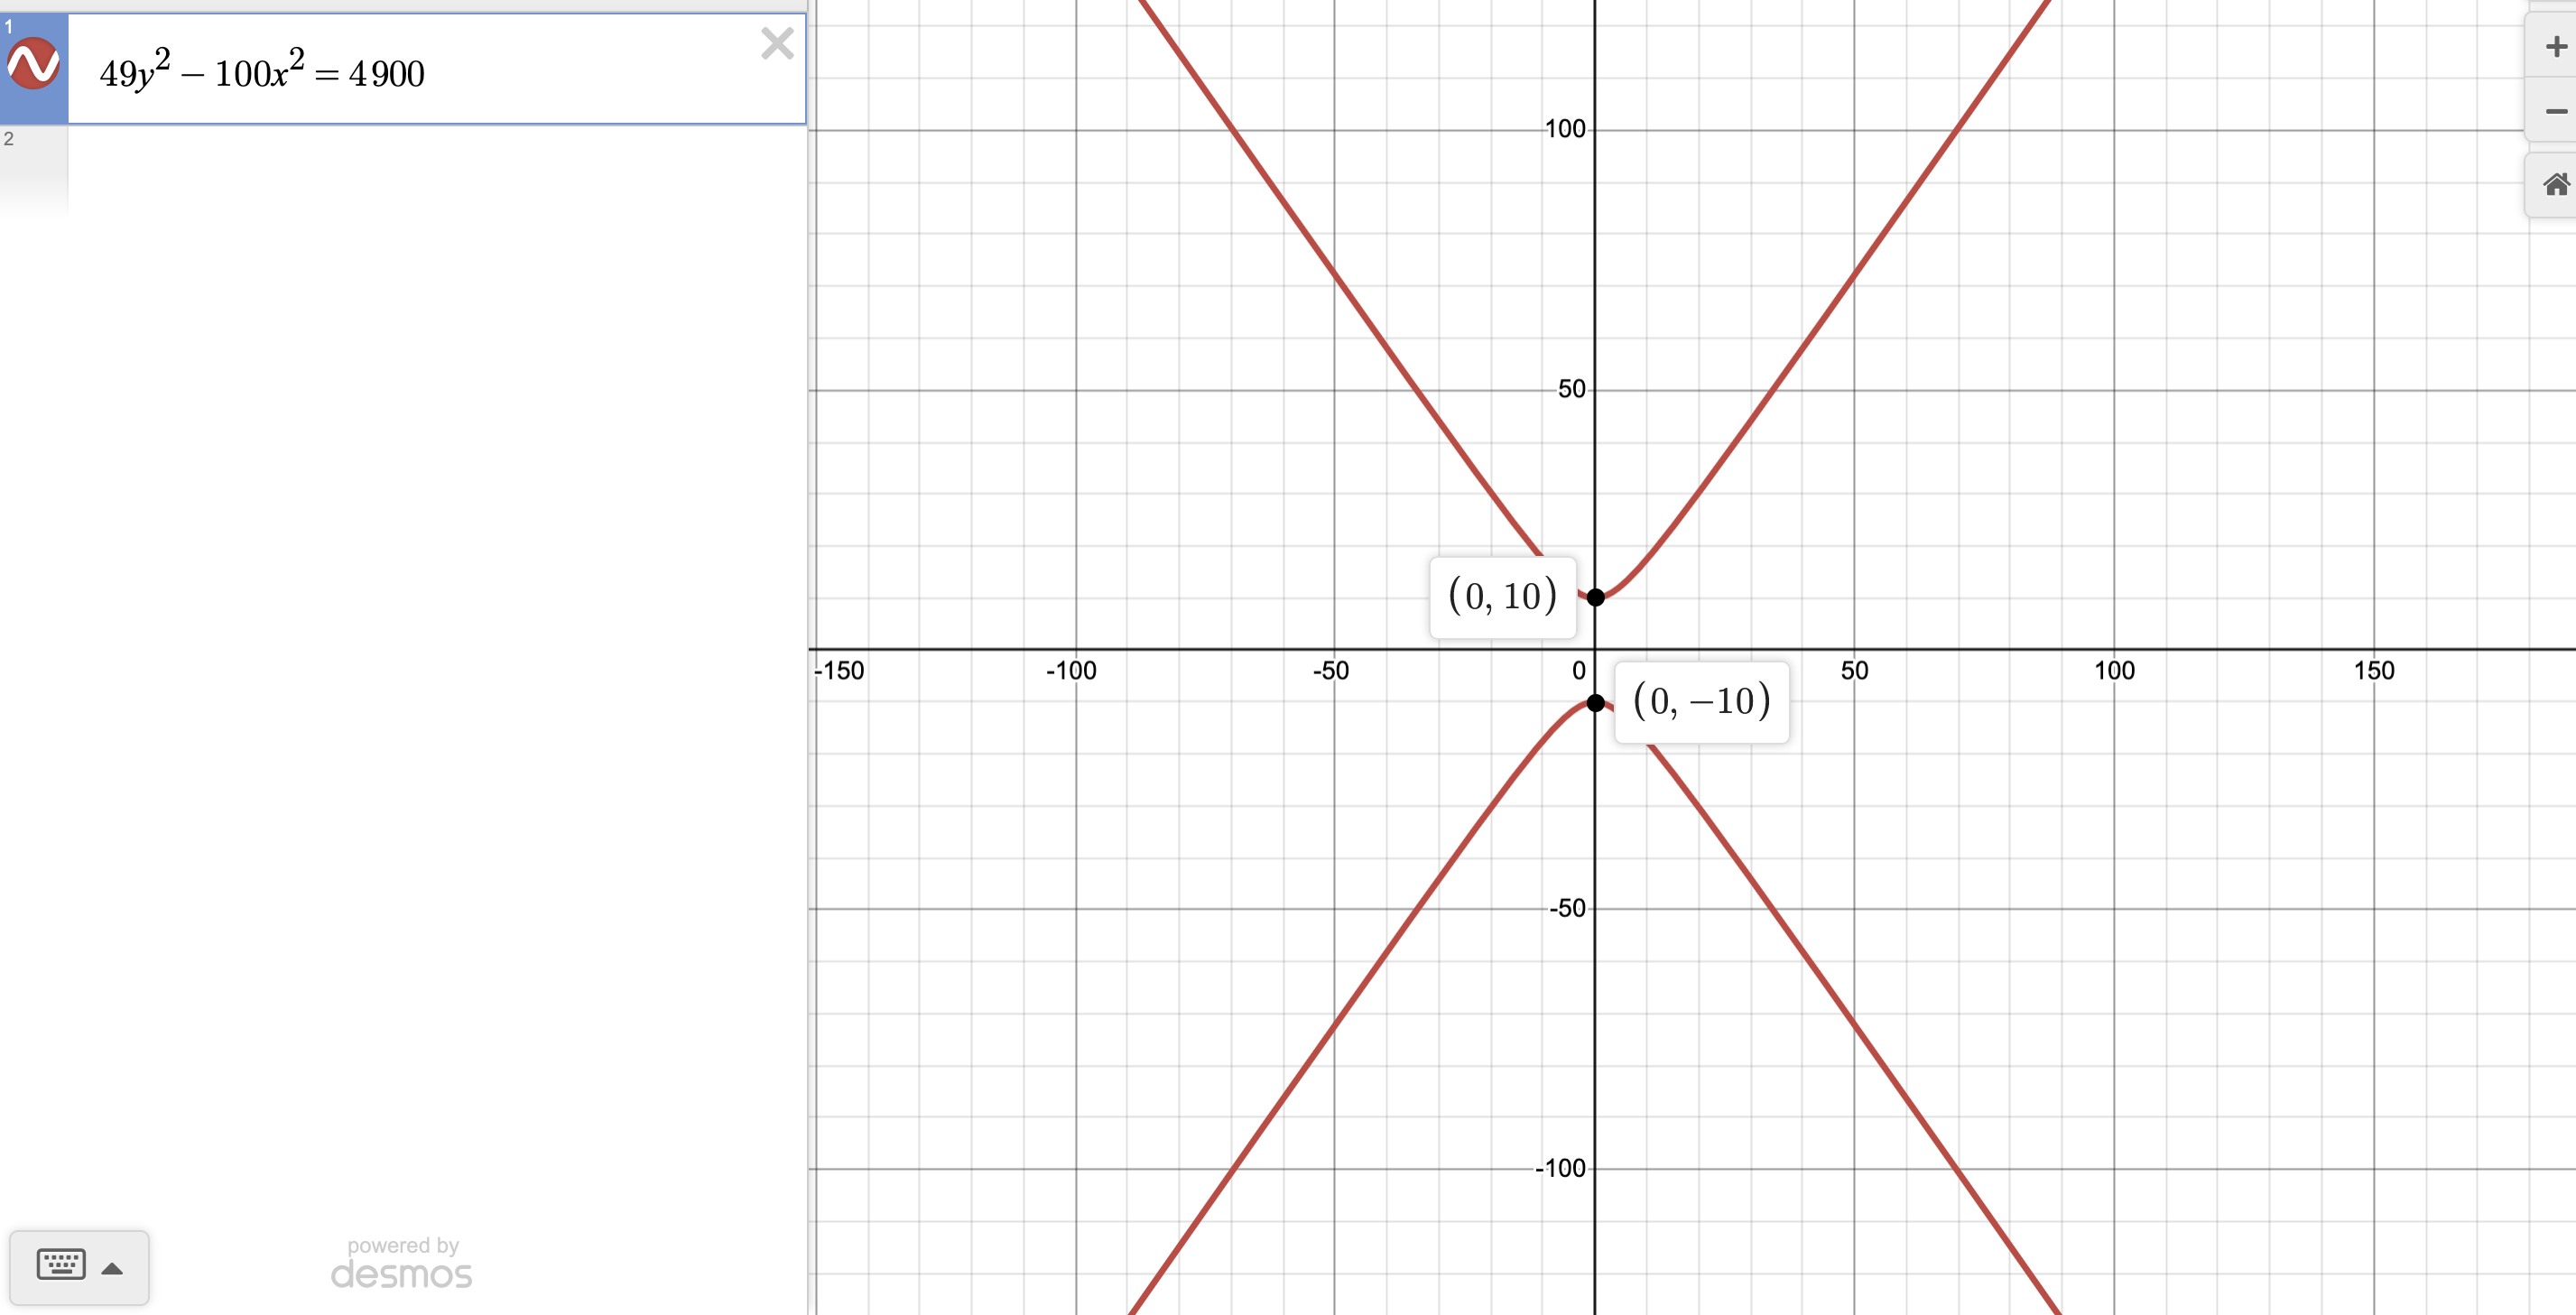
\includegraphics[width = 4in]{14}

\section*{15}
We are given the equation \[ 45y^2-200x^2=1800 \] \[ \frac{y^2}{40}-\frac{x^2}{9}=1 \] meaning $a=\sqrt{40}=2\sqrt{10}$. Because the $y^2$ term comes first, 
the transverse axis is vertical. Thus the vertices are $(0,\pm 2\sqrt{10})$. B

\section*{23}
We are given the foci $(0,\pm 4\sqrt{5})$ and the vertices $(0,\pm 4)$. Thus the transverse axis is vertical, $c=4\sqrt{5}$, and $a=4$. Then:
\[ (4\sqrt{5})^2=4^2+b^2 \]
\[ b=8 \] meaning the equation for the hyperbola is $\frac{y^2}{16}-\frac{x^2}{64}=1$.

\section*{24}
We are given the foci $(0,\pm 3)$ and the vertices $(0,\pm 2\sqrt{2})$. Thus the transverse axis is vertical, $c=3$, and $a=2\sqrt{2}$. Then:
\[ 3^2=(2\sqrt{2})^2+b^2 \]
\[ b=1 \] meaning the equation for the hyperbola is $\frac{y^2}{(2\sqrt{2})^2}-\frac{x^2}{1^2}=\frac{y^2}{8}-\frac{x^2}{1}=1$.

\section*{25}
We are given the foci $(\pm 3\sqrt{6},0)$ and the vertices $(\pm 2,0)$. Thus the transverse axis is horizontal, $c=3\sqrt{6}$, and $a=2$. Then:
\[ (3\sqrt{6})^2=2^2+b^2 \] \[ b^2=50 \] meaning the equation for the hyperbola is $\frac{x^2}{4}-\frac{y^2}{50}=1$.

\section*{26}
We are given the foci $(0,\pm 6\sqrt{3})$ and the vertices $(0,\pm 8)$. Thus the transverse axis is vertical, $c=6\sqrt{3}$, and $a=8$. Then:
\[ (6\sqrt{3})^2=8^2+b^2 \] \[ b^2=44 \] meaning the equation for the hyperbola is $\frac{y^2}{64}-\frac{x^2}{44}=1$. C

\section*{27}
We are given the equation $\frac{x^2}{25}-\frac{y^2}{49}=1$, meaning $a=\sqrt{25}=5$, $b=\sqrt{49}=7$, and because the term with $x^2$ in it comes first, the tranvserse 
axis is horizontal. Thus the asymptotes are $y=\pm\frac{5}{7}$. Also, the vertices are $(\pm 5,0)$:\newline
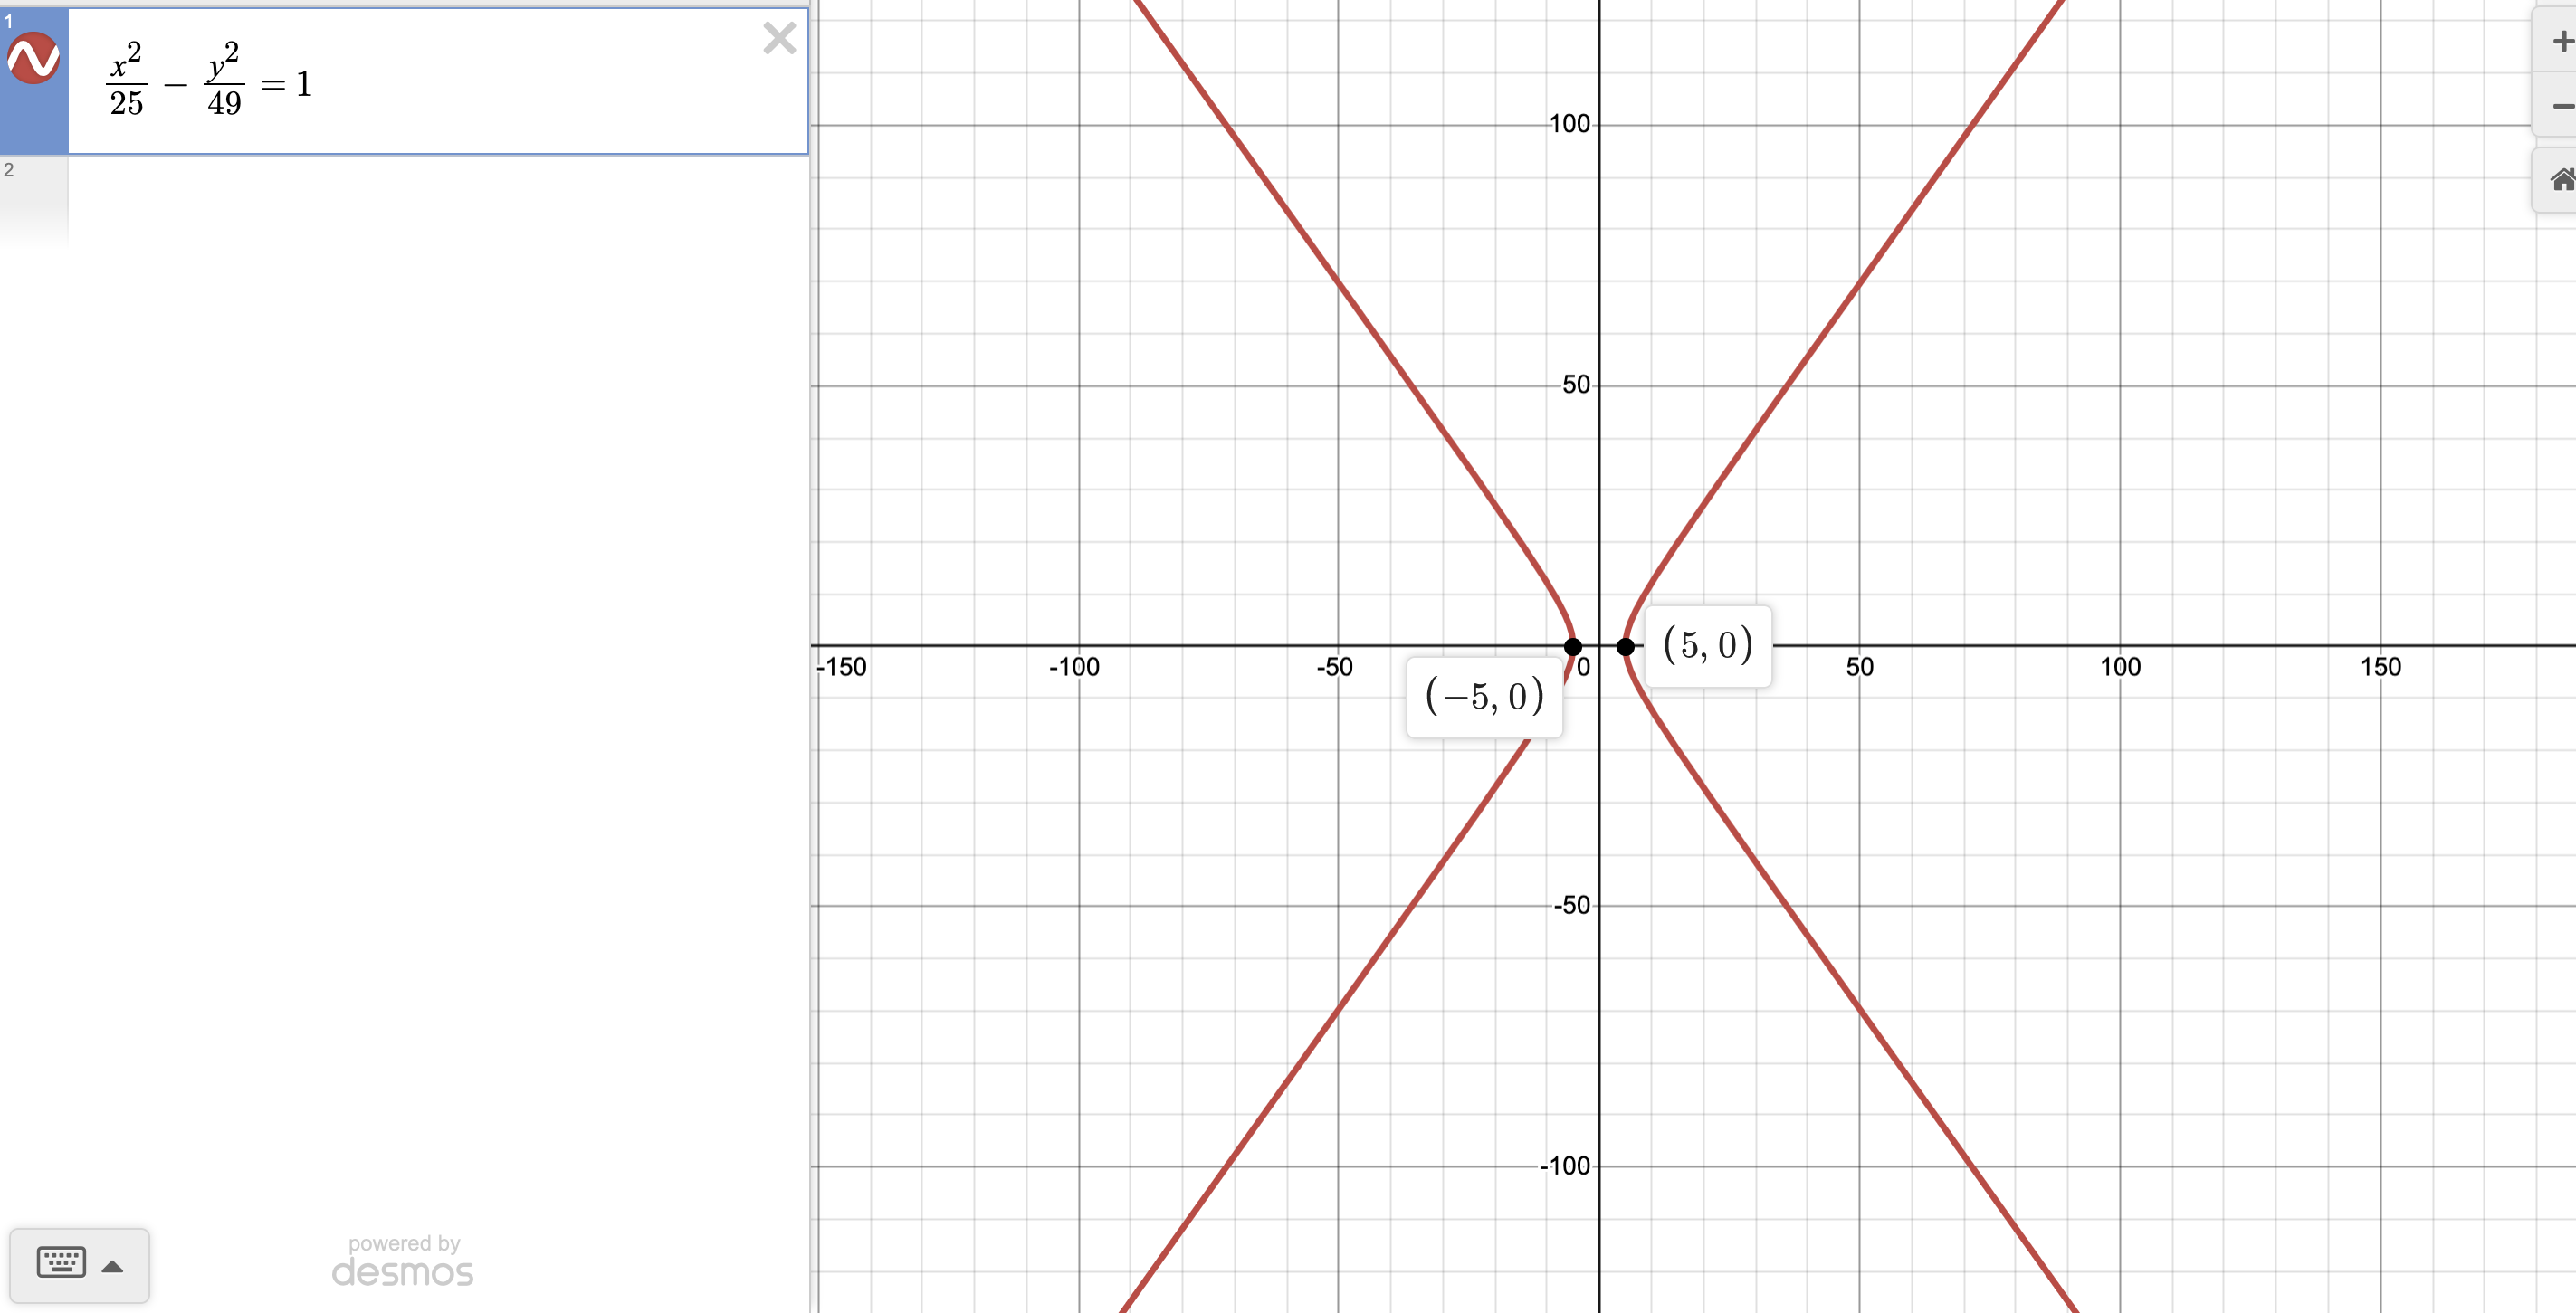
\includegraphics[width = 4in]{27}

\section*{28}
We are given the equation $y^2=18x$, meaning this is a parabola where $p=\frac{18}{4}=\frac{9}{2}$, and thus the focus is $(\frac{9}{2},0)$, the directrix 
is $x=-\frac{9}{2}$, and the axis of symmetry is $y=0$:\newline
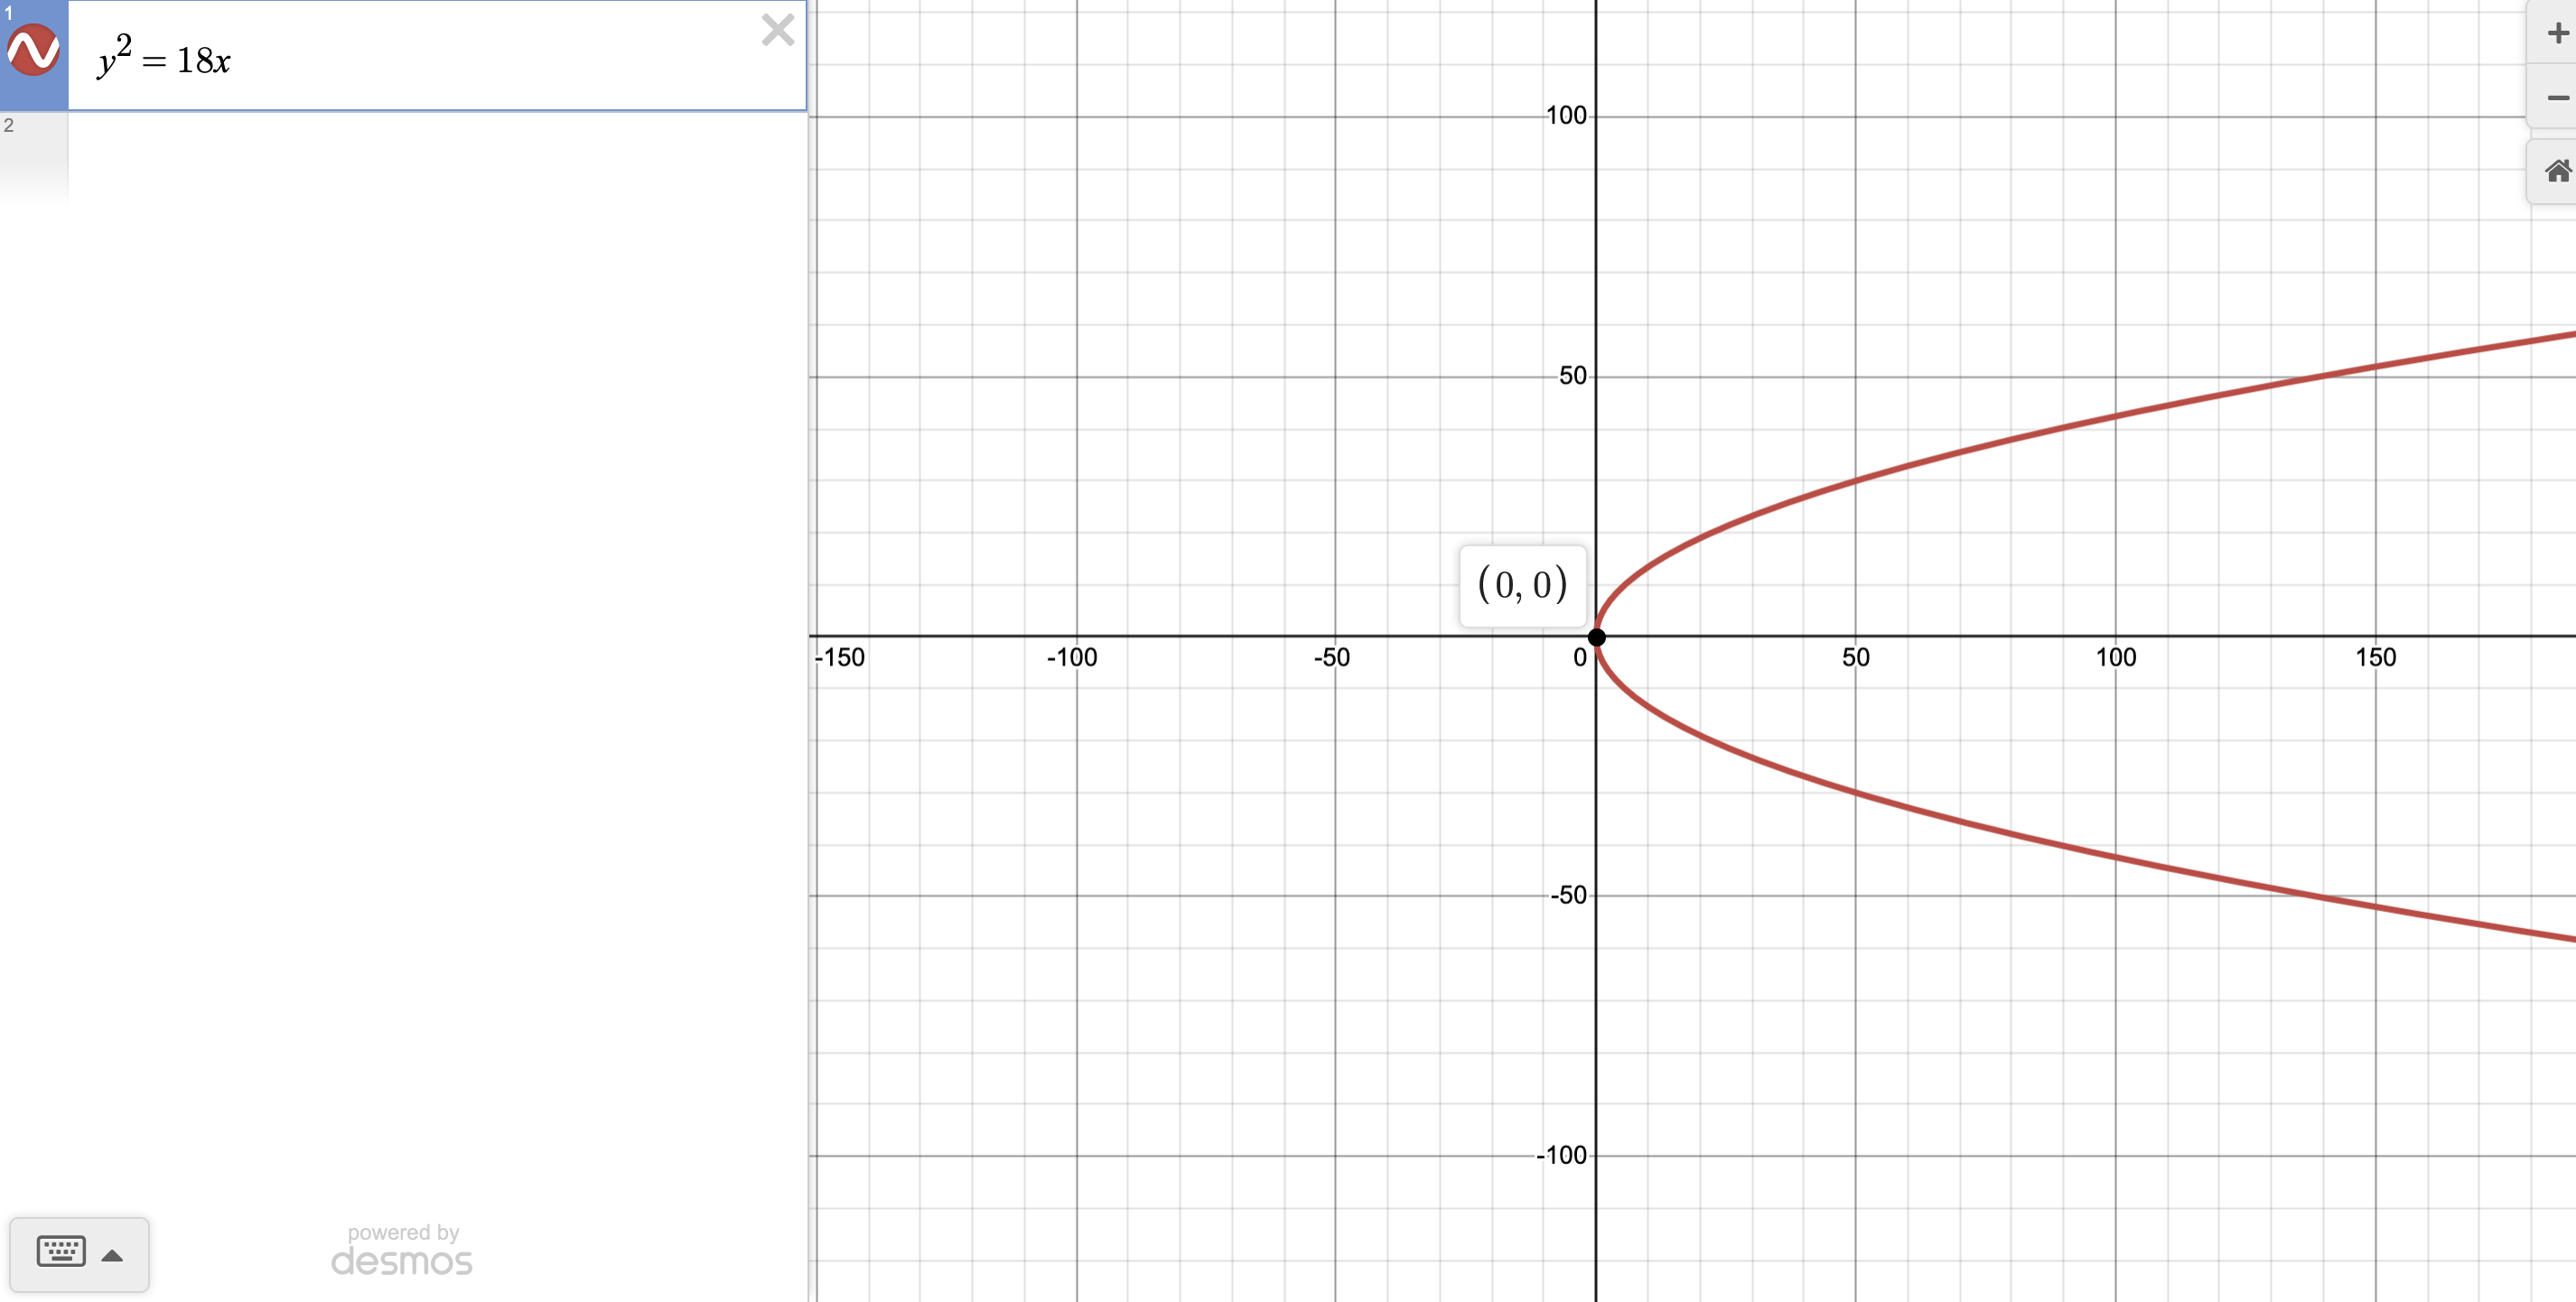
\includegraphics[width = 4in]{28}

\section*{29}
We are given the equation \[ 48x^2+12y^2=48 \] \[ x^2+\frac{y^2}{4}=1 \] meaning this is an ellipse with $b=\sqrt{1}=1$, $a=\sqrt{4}=2$, and with a vertical major axis.
Hence the vertices are $(0,\pm 2)$ and the co-vertices are $(\pm 1,0)$:\newline
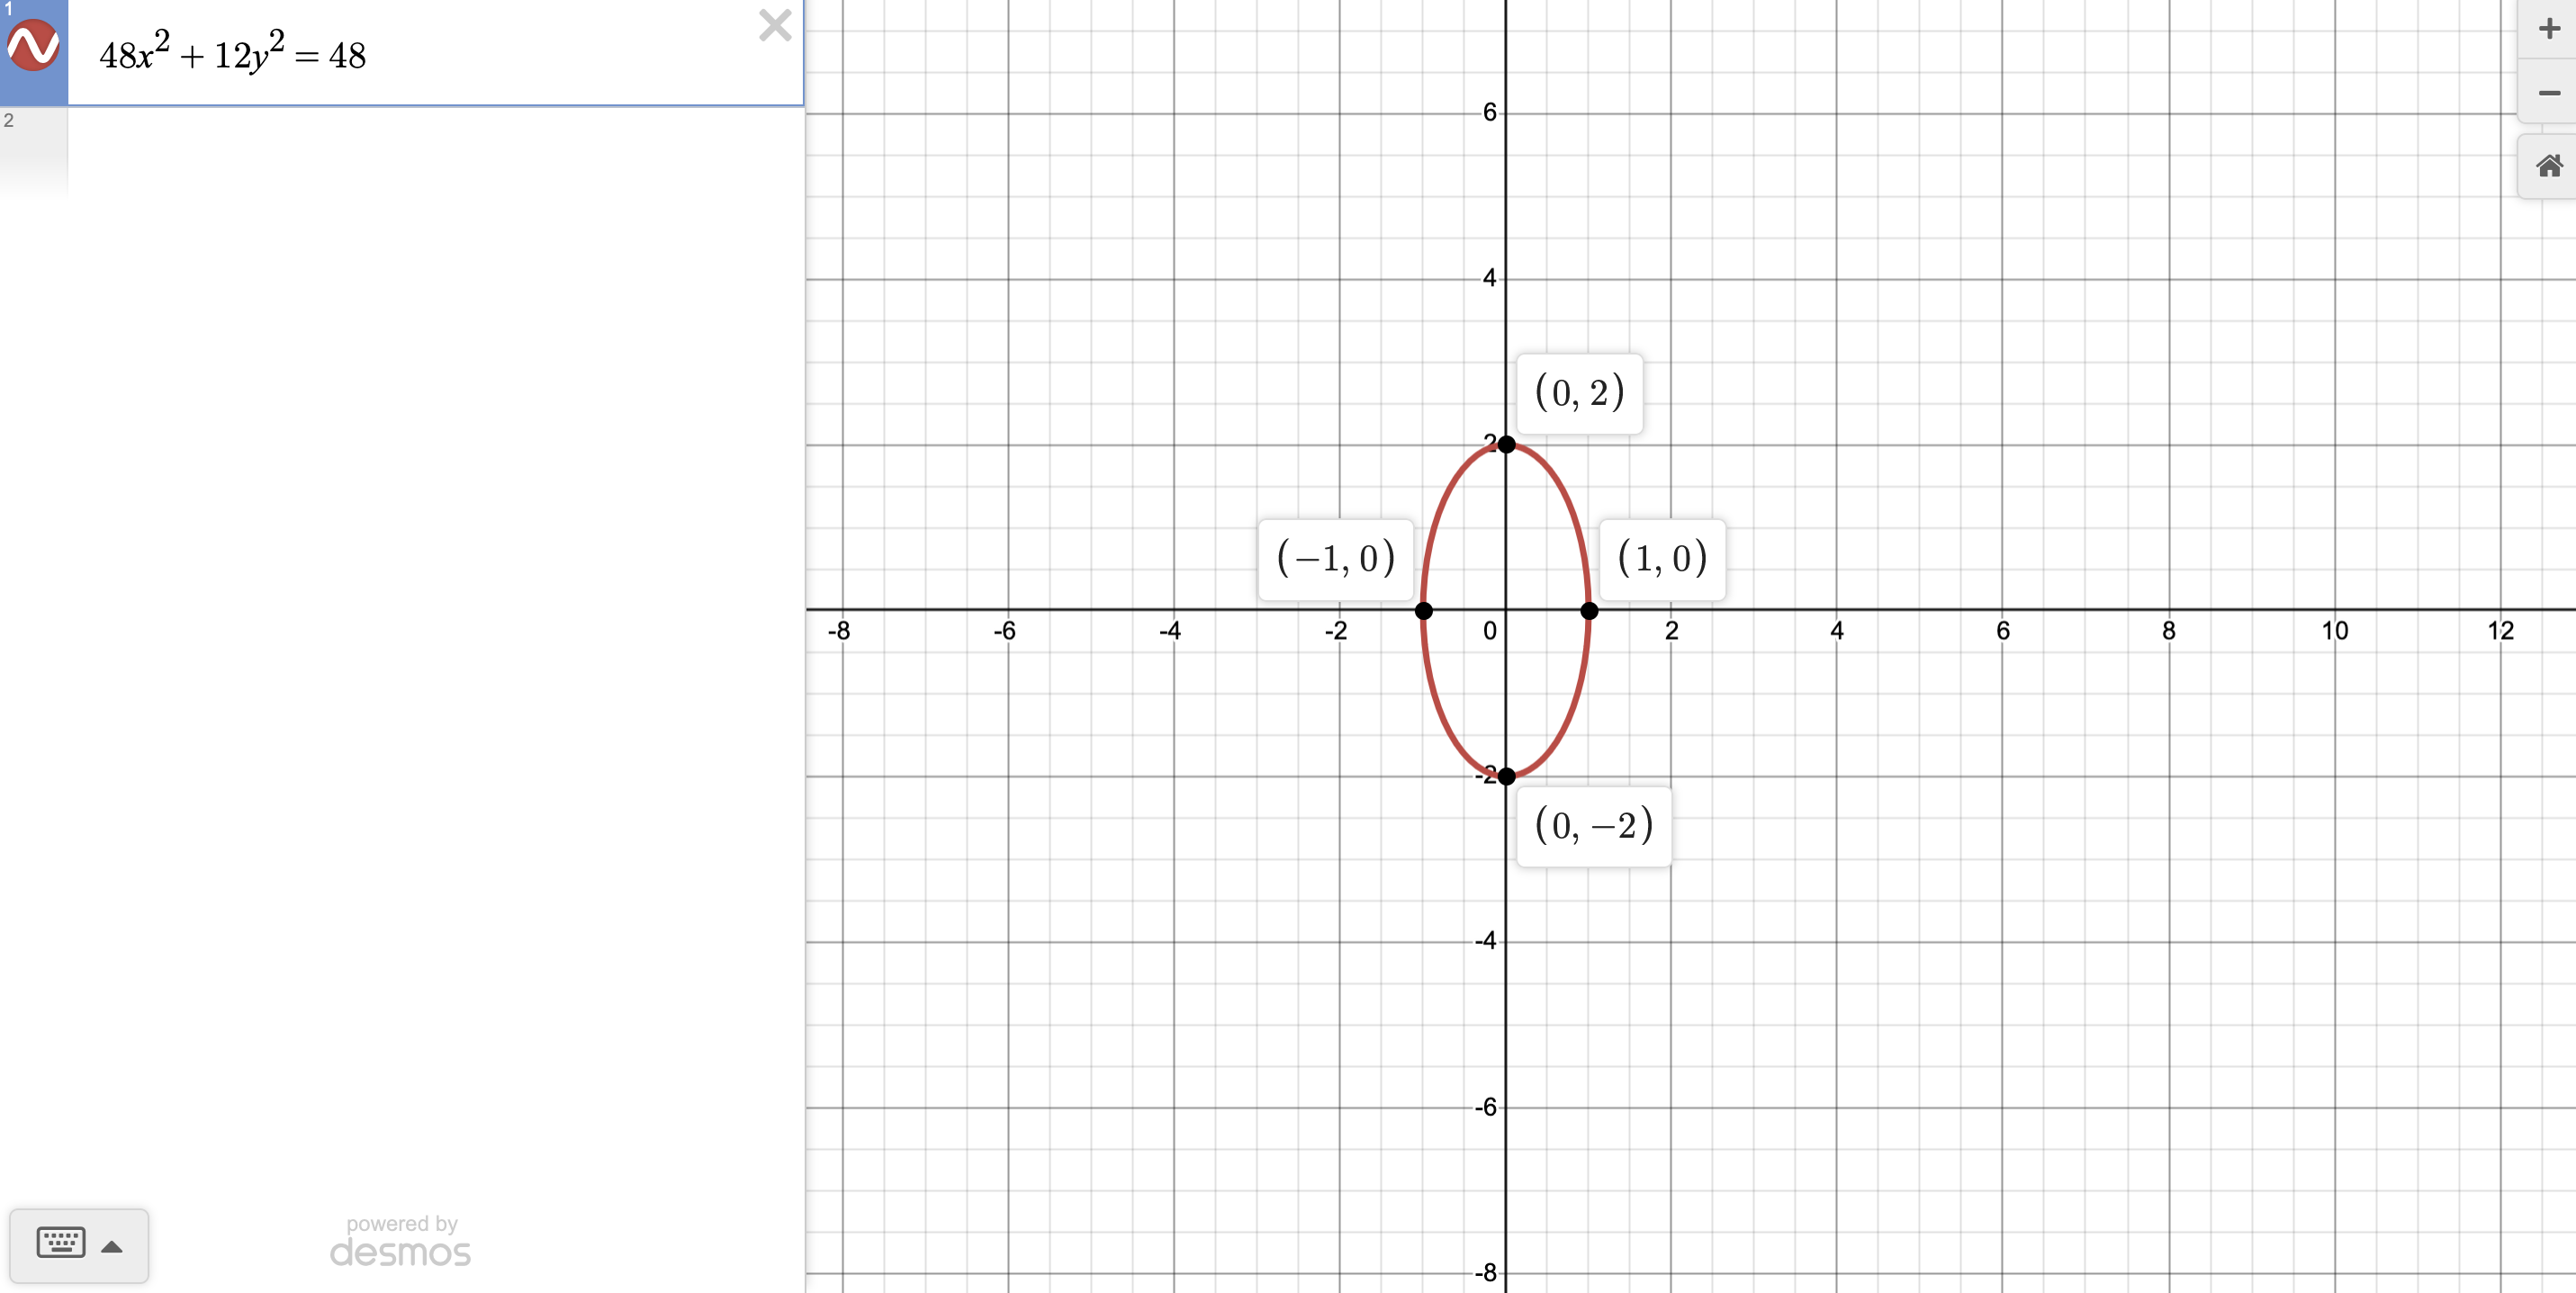
\includegraphics[width = 4in]{29}

\section*{32}
We are given the equation \[ 18x^2+18y^2=288 \] \[ x^2+y^2=4^2 \] meaning we this is a circle centered at the origin with a radius of 4:\newline
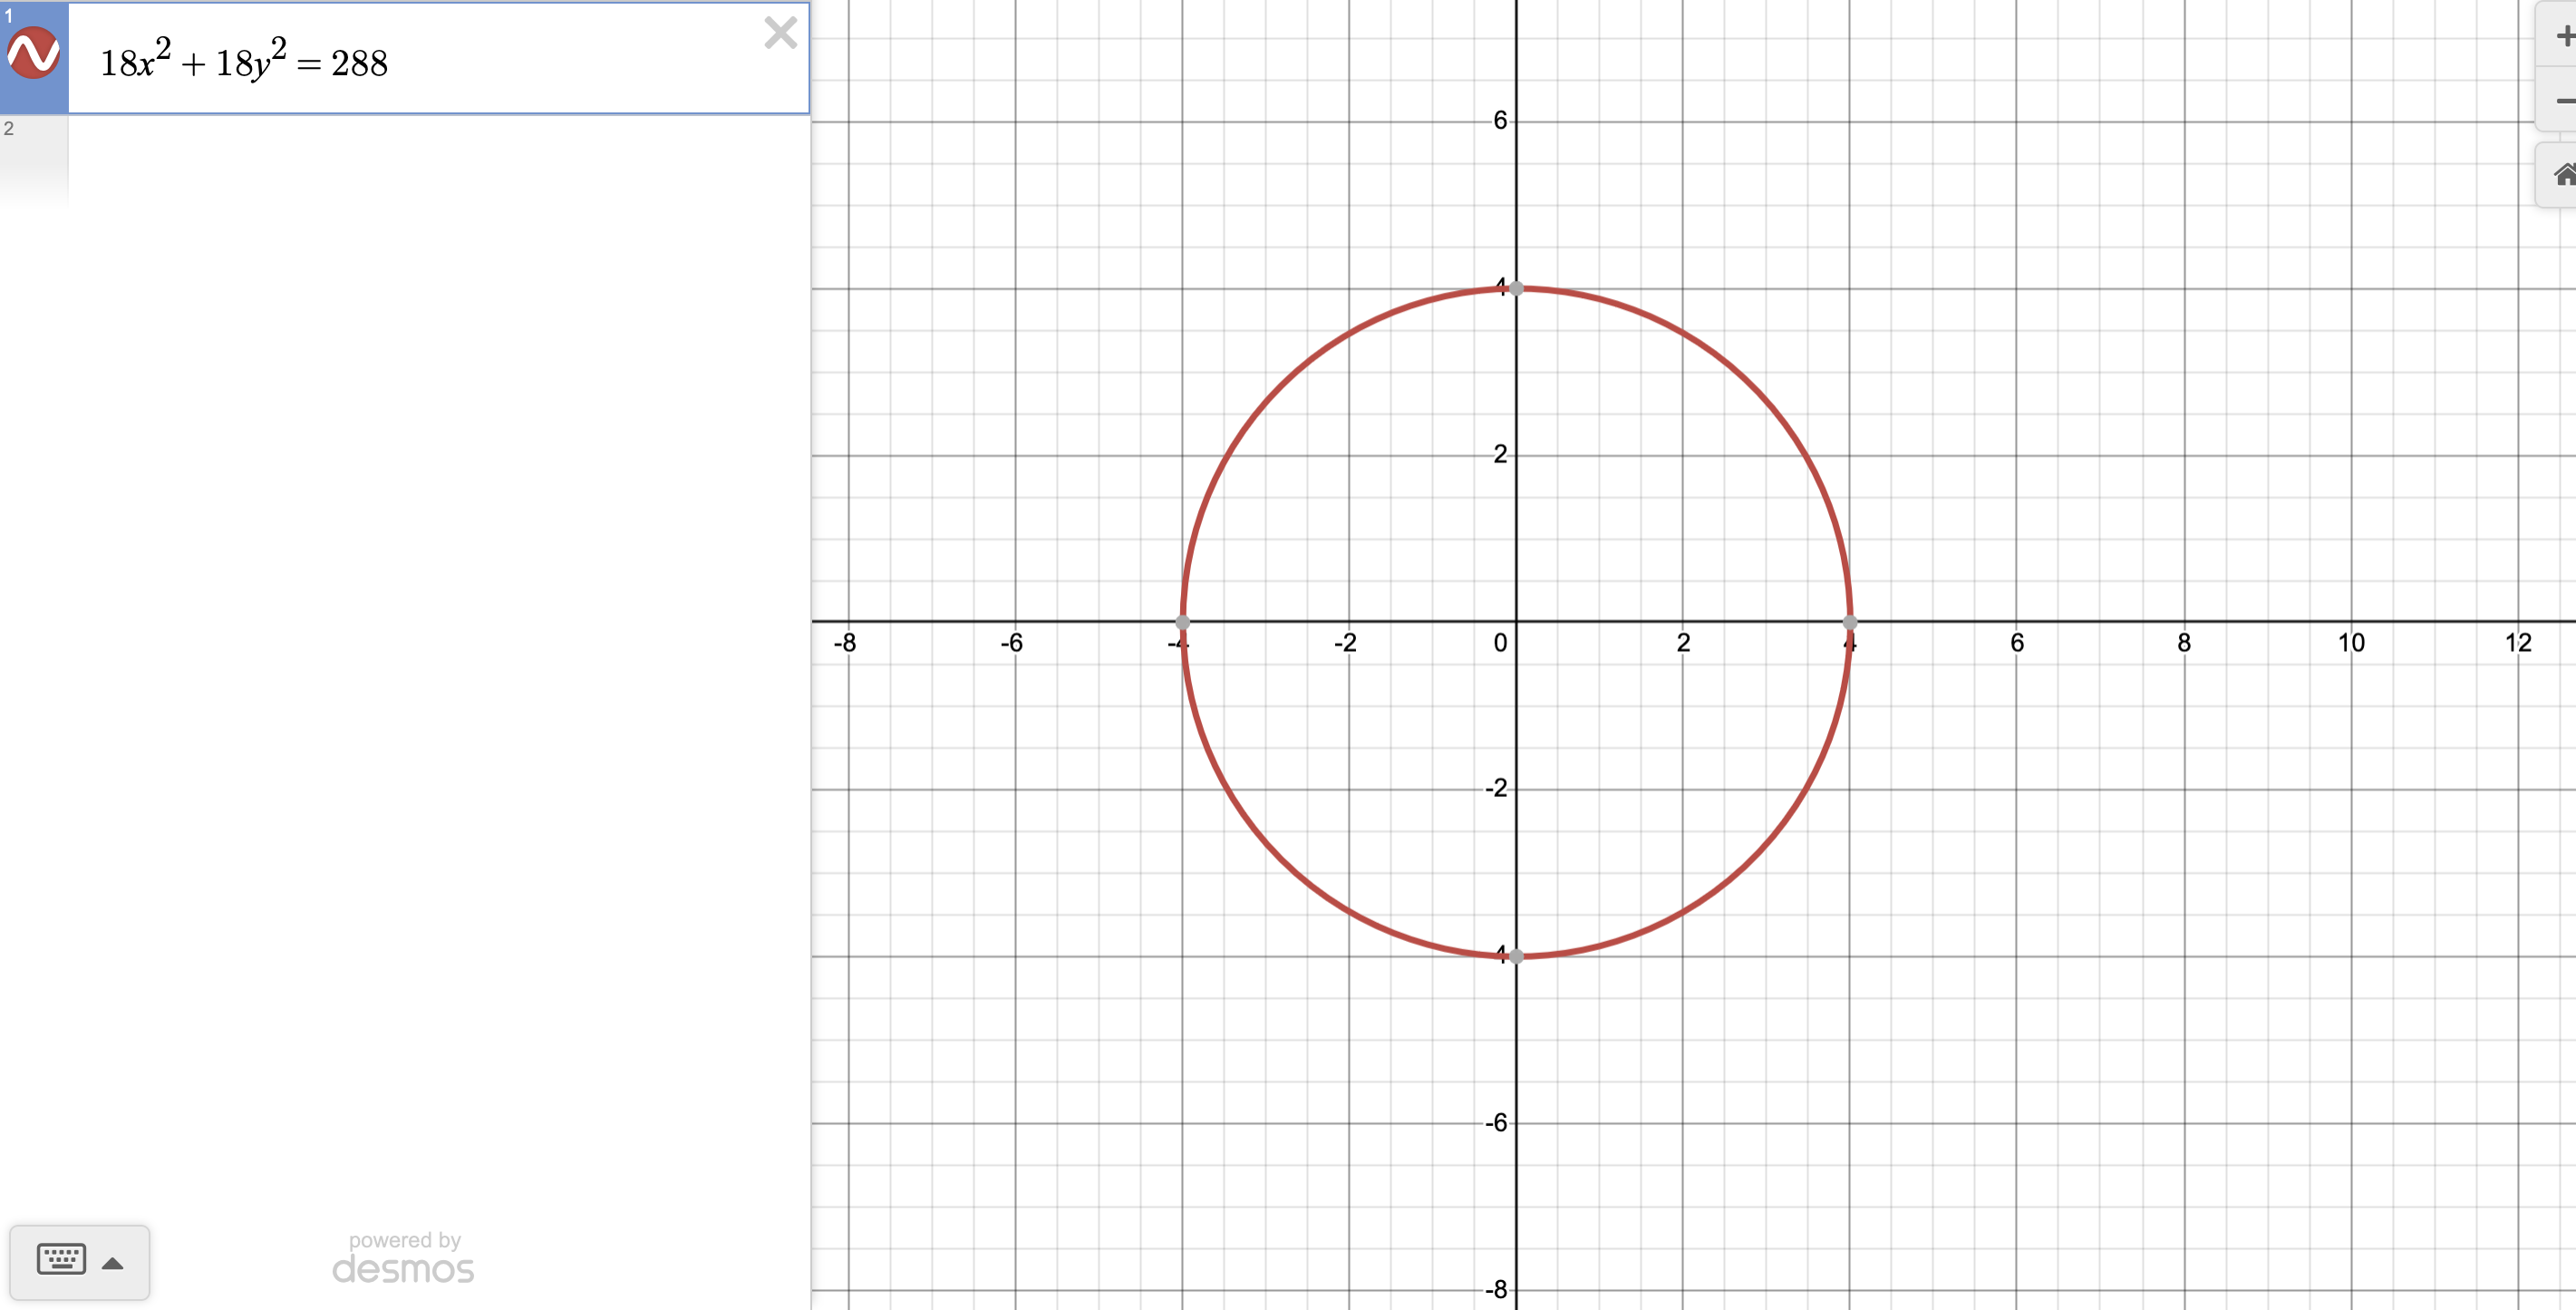
\includegraphics[width = 4in]{32}

\section*{34(a)}
We are given the equation \[ \frac{y^2}{15}-\frac{x^2}{30}=1 \] \[ \frac{y^2}{15}=\frac{x^2}{30}+1 \]
\[ y^2=\frac{x^2}{2}+15 \] \[ y=\pm\sqrt{\frac{x^2}{2}+15} \] Thus we can enter the two equations 
$y=\sqrt{\frac{x^2}{2}+15}$ and $y=-\sqrt{\frac{x^2}{2}+15}$ to graph the hyperbola.

\section*{36}
By the definition of a hyperbola, we know that $|d_2-d_1|$ is constant. Looking at the diagram to the right, we can see that the point $(a,0)$ is on the hyperbola. 
For $(a,0)$, the difference of the distances is $|(a+c)-(c-a)|=|2a|$. Because $a>0$, $|2a|=2a$. Thus we have shown that $|d_2-d_1|=2a$.

\section*{37}
We are given a hyperbola with foci at $(\pm 2,0)$ and such that the difference in the distances from a point $(x,y)$ on the hyperbola to the foci is 2. Because the 
foci are of the form $(\pm c,0)$, we know that the vertices are also of the form $(\pm a,0)$ (that is, the transverse axis is horizontal). 
Thus we have two points on the hyperboala: $(-a,0)$ and $(a,0)$. The distance from $(-a,0)$ to $(-c,0)$ is:
\[ \sqrt{(-a-c)^2}=-a-c \] and the distance from $(-a,0)$ to $(c,0)$ is \[ \sqrt{(-a+c)^2}=-a+c \] Thus the difference in distances is
$|(a-c)-(-a+c)|=2a$. Thus $2a=2$ and $a=1$. Hence:
\[ 2^2=1^2+b^2 \] \[ b^2=3 \] and thus the equation of the hyperbola is \[ x^2-\frac{y^2}{3}=1 \] Note that the answer to this problem did not require using 
the distance formula; we could have simply used the result of the previous problem. 

\section*{38}
We are given $a=33$ and $c=56$, and that the transverse axis is horizontal. Then:
\[ 56^2=33^2+b^2 \] \[ b^2=2047 \] and thus the equation of the hyperbola is $\frac{x^2}{56^2}-\frac{y^2}{2047}=1$.

\section*{39}
We are given $a=\frac{\sqrt{2}}{2}$ and $b=\frac{\sqrt{3}}{2}$. Thus:
\[ (\frac{\sqrt{3}}{2})^2=(\frac{\sqrt{2}}{2})^2+b^2 \]
\[ b^2=\frac{3}{4}-\frac{2}{4}=\frac{1}{4} \] \[ b=\frac{1}{2} \] meaning the equation of the hyperboal is (because we are given the transverse axis is 
horizontal) $\dfrac{x^2}{\frac{2}{4}}-\frac{y^2}{\frac{1}{4}}=1$, that is, \[ 2x^2-4y^2=1 \]

\section*{41}
(a): We are given that the building has a hyperbolic cross section. We are imagining that we overlaid a grid on the diagram with the origin at $O$. Thus, because we 
are given that $O$ is on a part of the roof that is 61 ft, we know that $a=\frac{61}{2}$. Thus the coordinate of point $A$ is $(\frac{61}{2},0)$. To find $B$, we simply need 
to find what the positive endpoint corresponding to the 170 ft. segment is. That endpoint is $(\frac{170}{2}=85,-40)$ (because that segment is forty feet below the center). 
Thus $B=(85,-40)$.


(b): We know that $(85,-40)$ is on the hyperbola, and we know $a$, meaning:
\[ \frac{85^2}{(\frac{61}{2})^2}-\frac{(-40)^2}{b^2}=1 \]
\[ -\frac{1600}{b^2}=1-\frac{7225}{930.25} \]
\[ -\frac{1600}{b^2}=-\frac{6294.75}{930.25} \]
\[ 1600=\frac{6294.75}{930.25}b^2 \]
\[ b=\sqrt{\frac{1488400}{6294.75}} \]
Thus an equation to model the hyperbola is:
\[ \dfrac{x^2}{(\frac{61}{2})^2}-\dfrac{y^2}{\frac{1488400}{6294.75}}=1 \]


(c): We know that one of the endpoints of the roof which is on the hyperbola has an (because it is 84 ft) $x$-coordinate of $42$, meaning:
\[ \dfrac{42^2}{(\frac{61}{2})^2}-\dfrac{y^2}{\frac{1488400}{6294.75}}=1 \]
\[ -y^2=(1-\frac{1764}{930.25})\times\frac{1488400}{6294.75} \]
\[ y=\sqrt{-\left((1-\frac{1764}{930.25})\times\frac{1488400}{6294.75}\right)} \]
\[ \approx 14.56 \] Thus the height of the roof is about $14.56+40=54.56$ ft.

\section*{42}
(a): We know that $\pi y^2-\pi x^2=600$, that is, $\pi(y^2-x^2)=600$, as we were given that a maximum of 600 square feet of concrete could be used.


(b):
\begin{center}
\begin{tabular}{l|l|l|l|l}
$x$ & $1$ & $2$ & $3$ & $4$ \\
$y$ & $\sqrt{\frac{600}{\pi}+1}$ & $\sqrt{\frac{600}{\pi}+4}$ & $\sqrt{\frac{600}{\pi}+9}$ & $\sqrt{\frac{600}{\pi}+16}$
\end{tabular}
\end{center}


(c): \newline 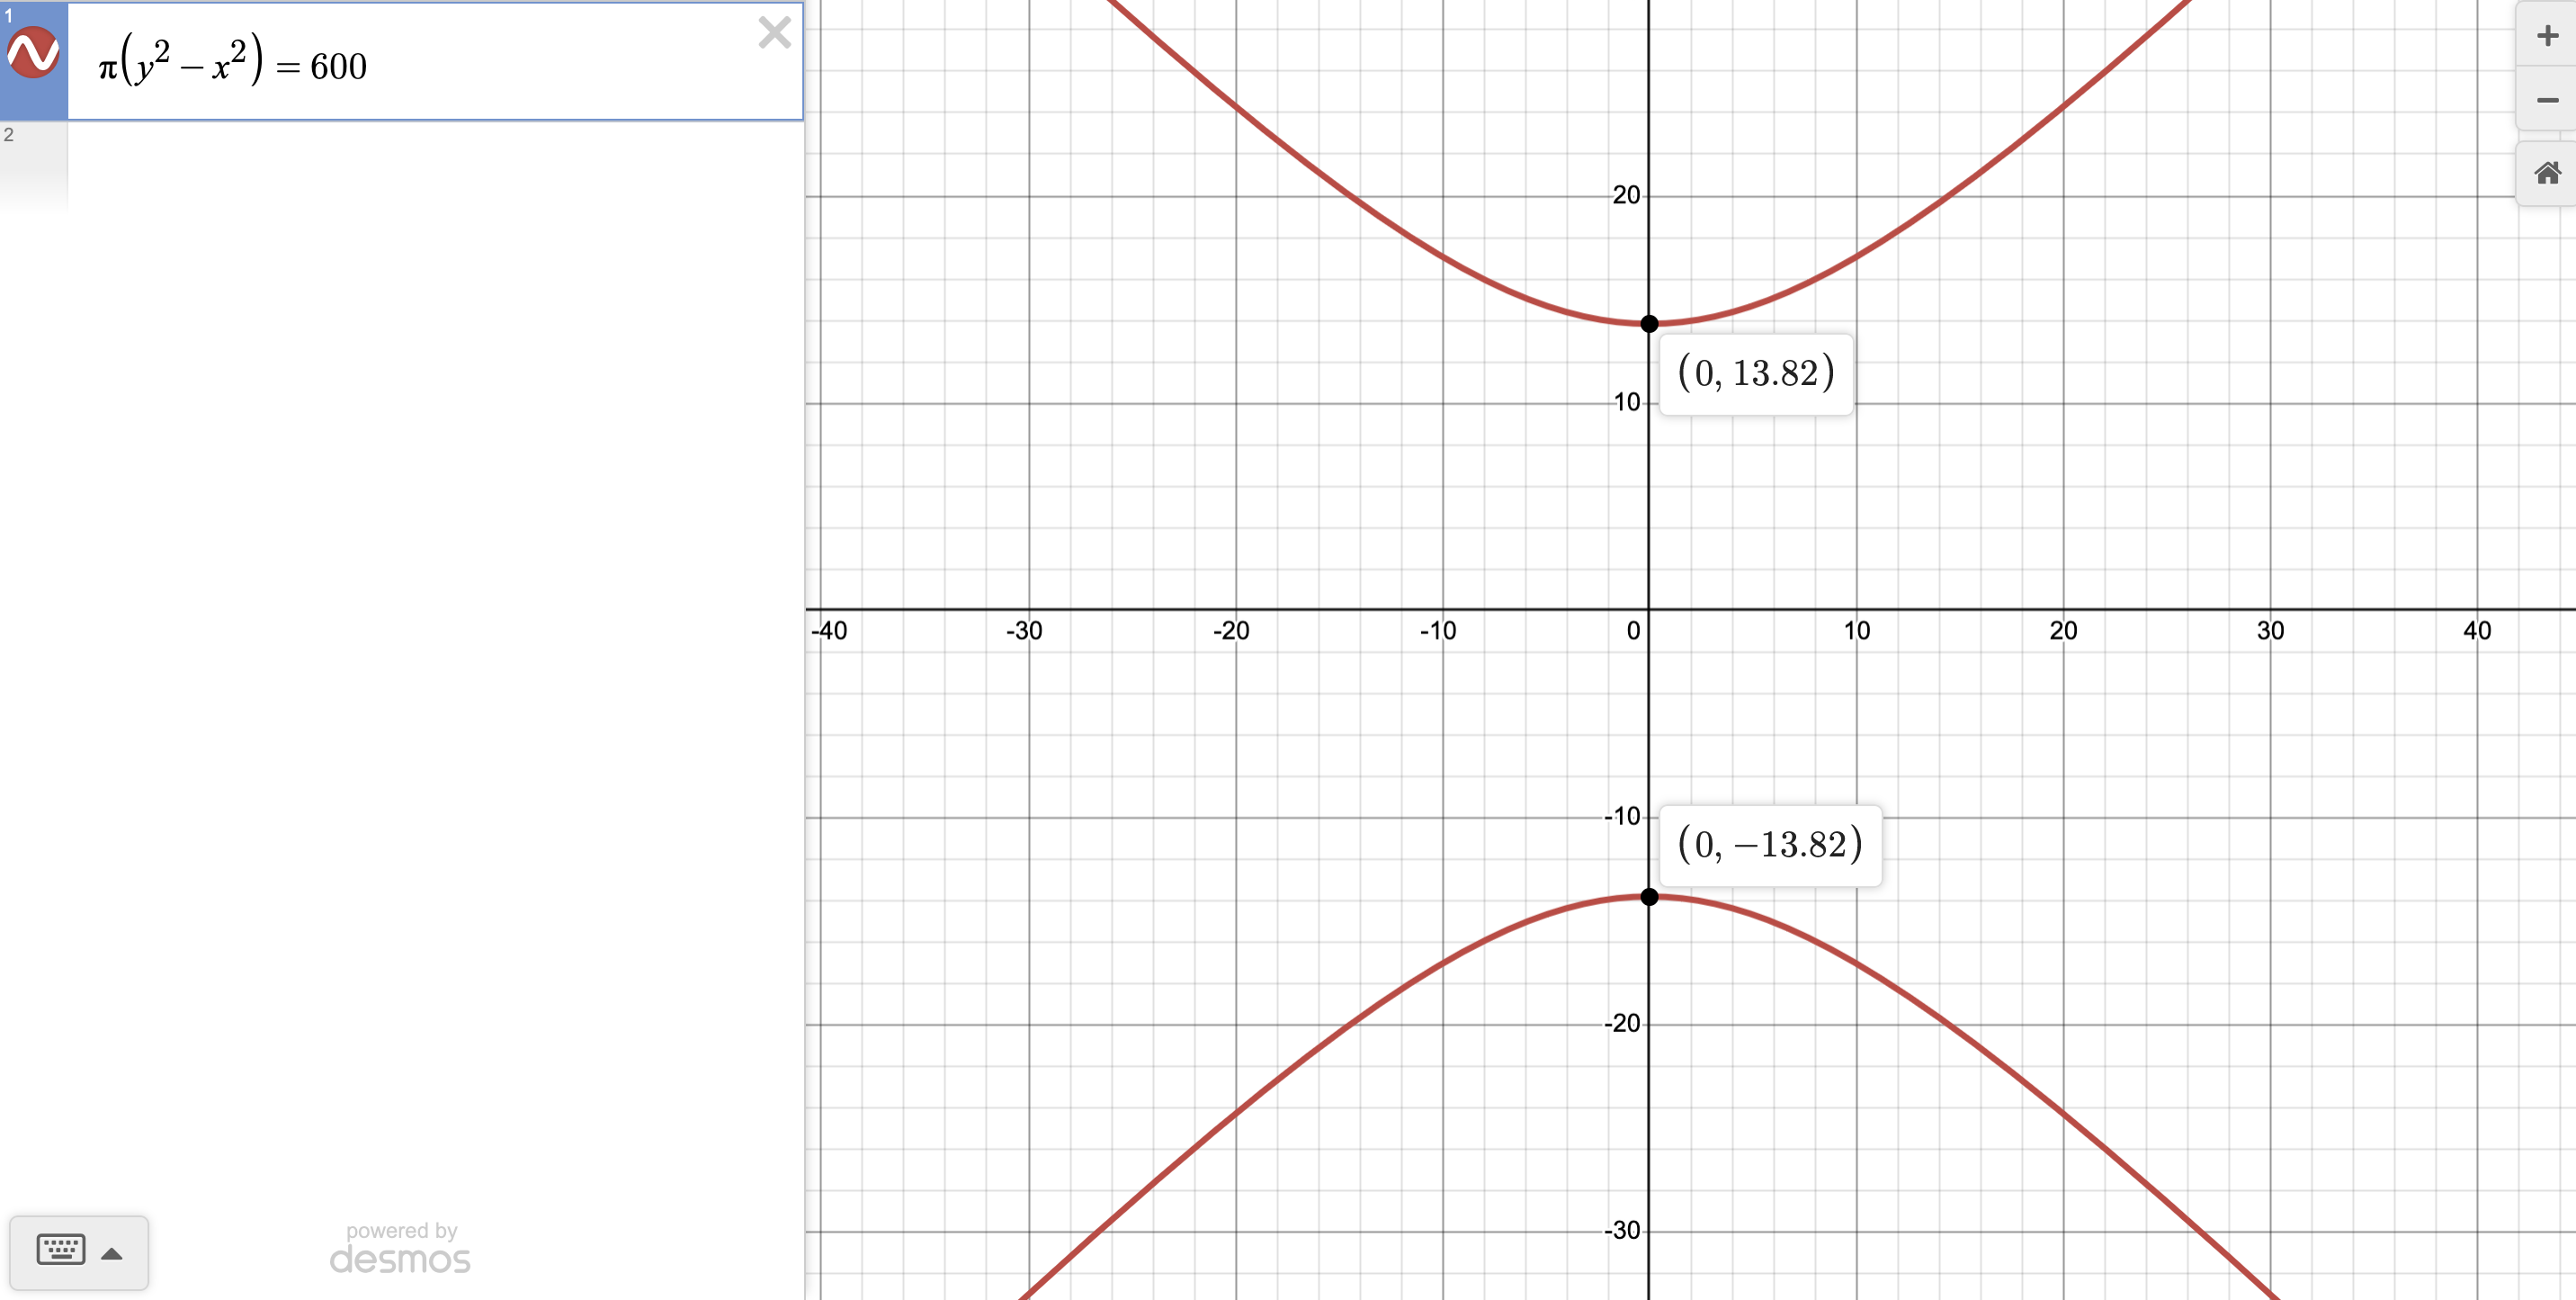
\includegraphics[width = 4in]{42}


(d): As both $x$ and $y$ increase, $y+x$ increases. Now, recall that from part (a), we know that:
\[ \pi(y^2-x^2)=600 \]
\[ \pi(y+x)(y-x)=600 \]
\[ y-x=\frac{600}{(y+x)\pi} \]
Because $\frac{600}{(y+x)\pi}$ decreases as $y+x$ increases, and we know that $y+x$ increases as both $x$ and $y$ increase, it follows that 
$y-x$ decreases as both $x$ and $y$ increase.


\section*{43}
(a): We are given that $a=4$ and $c=6$, meaning:
\[ 36=16+b^2 \] \[ b^2=20 \] thus meaning an equation for the hyperbola is $\frac{x^2}{16}-\frac{y^2}{20}=1$. 


(b):
The intersection points are the points when the circles intersect. We can consider the part of the hyperbola going in the positive direction. Here, the intersection at the vertex occurs 
when the circles $(x-6)^2+y^2=4$ and $(x+6)^2+y^2=100$ intersect. The second intersection occurs when the circles $(x-6)^2+y^2=9$ and $(x+6)^2+y^2=121$ intersect, and, in general, the 
$n$th intersection occurs when the circles $(x-6)^2+y^2=(2+n)^2$ and $(x+6)^2+y^2=(10+n)^2$ intersect. What this means is that the the distance between these points of intersection and the 
foci is just the radii of the circles. Thus the difference is $|(10+n)-(2+n)|=|8|=8$, therefore showing that the differences between the distances between the point of intersection and foci stay 
the same; hence this is a hyperbola.

\section*{44}
I was not able to solve this.

\end{document}
